\documentclass[a4paper,12pt]{article}

\usepackage[utf8]{inputenc}
\usepackage[english]{babel}
\usepackage{algorithm}
\usepackage{algpseudocode, biblatex}
\usepackage{comment}
\usepackage{amssymb,amsmath,amsthm}
\usepackage{graphicx}

\addbibresource{memory_pair.bib} 

% set the theorem styles according to the argument
\newtheorem{theorem}{Theorem}[section]
\newtheorem{lemma}[theorem]{Lemma}
\newtheorem{assumption}[theorem]{Assumption}
\newtheorem{definition}[theorem]{Definition}
\newtheorem{remark}[theorem]{Remark}

\title{Mo Memory, Mo Problems: Stream-Native Machine Unlearning}

\author{Kennon Stewart}

\begin{document}

\maketitle

\begin{abstract}

Machine unlearning work assumes a static, i.i.d training environment that doesn't truly exist. Modern ML pipelines need to learn, unlearn, and predict continuously on production streams of data. We translate the notion of the batch unlearning scenario to the online setting using notions of regret, sample complexity, and deletion capacity. We further tighten regret bounds to a logarithmic $\mathcal{O}(\ln{T})$, a first for a machine unlearning algorithm. And we swap out an expensive Hessian inversion with online variant of L-BFGS optimization, removing a memory footprint that scales linearly with time. Such changes extend the lifespan of an ML model before expensive retraining, making for a more efficient unlearning process.

\end{abstract}


\section{Introduction}
\label{sec:intro}

Industry has transitioned to a serverless and event-based cloud architecture for software. State changes are communicated with ACID transactions that collectively contain as much information as the data store itself. As opposed to waiting for batch pipelines to process and aggregate the data into a structured state, developers need stream-native learners that can learn continuously from the source while performing inference.

The problem is made more interesting by recent legislation. The European Union's General Data Protection Regulation provides users the right to be forgotten: to have their data summarily deleted from a company's servers, and the effect of such data removed from a statistical model. Statistical models not only need to learn on a stream of unstructured data, but also unlearn their training points just as easily without accuracy loss, known as catastrophic forgetting.

We provide a framework for online algorithms that encompasses both learning and unlearning. We build specifically for the case of distributed systems where learning and unlearning are \textbf{necessary, interleaved} operations used to refine model accuracy. We show that the memory pair meets state-of-the-art regret guarantees with a sublinear memory footprint particularly suited for online learning. It also satisfies $(\varepsilon,\delta)$-unlearning requirements, which makes it particularly suitable for the task of regulatory compliance.

Unlearning research has begun to address the privacy side.  The frameworks of Sekhari et al. and Qiao et al. provide provable $(\varepsilon,\delta)$ guarantees that a post-hoc deletion yields (in distribution) the same parameters as a fresh retrain \cite{Sekhari_Acharya_Kamath_Suresh_2021-03}.  However, both assume an offline model that never learns again after deletion. We assume a stream environment where deletions and insertions are events processed in sequence.

\section{Stream-Native Learning}
\label{sec:stream-native}

The next generation of ML systems must treat \textit{learning}, \textit{forgetting}, and \textit{predicting} as first-class, intertwined operations performed on a live data stream.  To this end we introduce the \textbf{Memory Pair} pipeline:

\begin{itemize}
    \item \textit{Stream-native learning:} A learner $A$ ingests each example $(x_{t},y_{t})$ and performs an $O(d)$ update in micro-seconds, maintaining only lightweight sketches instead of per-sample gradients.
    \item \textit{Deferred inference gate:} Predictions are withheld until the running sample count exceeds a theoretically derived sample-complexity threshold, ensuring the first answer is already PAC-competitive.
    \item \textit{Symmetric unlearning:} A paired algorithm $\bar{A}$ accepts deletion requests via the same API and issues a one-step \textit{negative} update that preserves the learner’s regret bound. The model is guaranteed to be within an arbitrary precision of the ideal cold-start model trained from scratch.
    \item \textit{Live deletion-capacity odometer:} Each unlearning step depletes the model's deletion capacity budget. When a model unlearns its capacity, the learner is flagged for retraining to preserve accuracy.
\end{itemize}

\subsection{Contributions}
\label{subsec:contributions}

We contribute a complete \emph{stream–native} learning–unlearning pipeline and its theoretical analysis:

\begin{enumerate}
    \item \textbf{Memory‐Pair framework.}  We introduce the first online algorithm that simultaneously (i) converges to the empirical-risk minimizer on a live data stream and (ii) provides $(\varepsilon,\delta)$-certified unlearning for every \textsc{delete} event.  The design works with interleaved \textsc{insert}, \textsc{delete}, and \textsc{predict} operations and stores only $\mathcal{O}(d\tau)$ curvature pairs. 
    
    \item \textbf{Sharper regret guarantees.}  Under strong convexity we prove a \(\mathcal{O}\!\bigl(G^{2}/(\lambda)\ln T\bigr)\) \emph{static} regret bound—the first logarithmic guarantee for certified unlearning—and extend it to a \(\mathcal{O}\!\bigl(G^{2}/(\lambda)\ln T + G P_T\bigr)\) \emph{dynamic} regret bound that adapts to distribution drift through the comparator path-length~\(P_T\).

    \item \textbf{Adaptive capacity and complexity bounds.}  Using an AdaGrad-style statistic \(S_T\) we derive closed-form $\gamma$-\emph{deletion capacity} and $\gamma$-\emph{sample complexity} formulas that tighten to \(\widetilde{\mathcal{O}}(\sqrt{T})\) in the worst case and improve automatically when gradients decay.

    \item \textbf{Lightweight privacy accounting.}  We embed a live \emph{deletion‐capacity odometer} that tracks the zCDP budget, guaranteeing that the model halts and retrains precisely when further unlearning would violate either privacy or regret guarantees.  
\end{enumerate}

\section{Preliminaries}
\label{sec:prelim}

The batch unlearning framework from Sekhari et al. provides the theoretical inspiration for true online unlearning \cite{Sekhari_Acharya_Kamath_Suresh_2021-03}. By focusing on population risk, they establish that unlearning with generalization guarantees is possible. However, their algorithm is designed for a static, i.i.d. world.

Our Memory Pair framework adapts these core ideas for a dynamic, online setting. We replace the assumption of i.i.d. data with a non-stationary stream, substitute the excess risk metric with the more robust notion of cumulative regret, and swap the expensive, offline Hessian-based update with a lightweight, stream-native L-BFGS approximation\cite{Mokhtari_Ribeiro_2014-09}. 

The Memory Pair is not just a generalization of the batch algorithm but a \textit{necessary evolution} designed to handle the continuous learning, forgetting, and inference demands of a live data stream.

We start by framing our learners within the online learning paradigm. Batch learning  minimizes the loss function evaluated over a static training set. We instead use the seminal notion of regret, which appropriately compares the online learner to the best possible model in hindsight for a particular realized sequence of events \cite{Cesa-Bianchi_Lugosi_2006}.

This demonstrates the key factor of the Sekhari paper. By requiring the model to satisfy population risk guarantees, the model is expected to perform well against some true but unknown parameter distribution. This is very similar to the case of online learning because the model's evaluation is continuous, and the descent is adjusted accordingly.

\begin{definition}[Online learner with vanishing average regret]
\label{def:online-learner}
Let $\mathcal W \subseteq \mathbb{R}^d$ be a convex hypothesis set and $\{\ell_t\}_{t=1}^\infty$ an arbitrary sequence of (not necessarily stationary) loss functions $\ell_t : \mathcal W \to \mathbb{R}_{\ge 0}$. An algorithm $\mathcal A$ that, after observing an outcome $(x_{t},y_{t})$, outputs a weight vector $w_t = \mathcal A(x_{1:t},y_{1:t}) \in \mathcal W$ is called an \emph{online learner} iff for every outcome sequence $\{(x_{t},y_{t})\}_{t=1}^\infty$ the \emph{average regret}
\[
  \frac{1}{n}\,R_n(\mathcal A)
  \;:=\;
  \frac{1}{n}
  \Bigl(
    \sum_{t=1}^{n}\ell_t(w_t)
    -
    \min_{w\in\mathcal W}\sum_{t=1}^{n}\ell_t(w)
  \Bigr)
\]
converges to zero,
i.e.
\[
  \frac{1}{n}\,R_n(\mathcal A)
  \;\xrightarrow[n\to\infty]{}\;0.
\]
\end{definition}

In the online setting, a model is expected not only to learn incrementally, but also process data deletion requests with some measure of guarantee. The unlearner must yield an unlearned model that is statistically indistinguishable from the retrained ideal. This tight, state-dependent relationship requires a unified framework where learning and unlearning procedures are tightly coupled.

It's also worth noting that the real-world is not necessarily stationary. The underlying distribution of data streams will show real-time shifts in the underlying parameter distribution. It's essential that the model learn these new distributions adaptively to maintain error guarantees.

We formalize the notion of a memory pair as a coupled learning-unlearning algorithm designed to operate on a stream of insertions and deletions. A valid memory pair must simultaneously guarantee learning accuracy constraints, unlearning fidelity, and the capacity to handle a certain number of deletions.

\begin{definition}[Memory Pair]
\label{def:memory-pair}

Let $\{E_t\}_{t=1}^{N}$ be an event stream where $E_{t}\in \{\texttt{insert}(x_{t},y_{t}),\texttt{delete}(u_{t})\}$.  
A pair of algorithms $(A,\bar A)$ with shared state $\theta_{t-1}$ acts as
$$
\text{learn step: }\theta_t = A(\theta_{t-1},E_t),\qquad
\text{unlearn step: }\bar\theta_t = \bar A(\theta_{t-1},E_t).
$$

Denote by $\tilde{\theta_{t}}$ the {\it ideal replay model}, i.e.\ the model
obtained by replaying all past \texttt{insert} events except those whose
indices have appeared in a prior \texttt{delete}.  
Fix an accuracy target $\gamma$, confidence $\delta$, privacy budget
$(\rho^{*},\delta^{*})$ in the sense of zCDP, and a deletion capacity
$m$.  Then $(A,\bar A)$ is a
\emph{$(\gamma,m,\rho^{*},\delta^{*})$-memory pair} if, for every
event stream and for every horizon $N$, the following hold:

\begin{enumerate}
\item[\textbf{(I)}] \textbf{Online accuracy.}  
      \(
      \Pr\!\bigl[\tfrac1N R_N(\theta)\le\gamma\bigr]\;\ge\;1-\delta.
      \)

\item[\textbf{(II)}] \textbf{\(\rho^{*}\)-zCDP online unlearning.}  
      For every measurable set $S\subseteq\mathcal{W}$ and every
      $t\!\le\!N$,
      $$
        D_\alpha\!\bigl(\bar\theta_t\!\parallel\!\tilde\theta_t\bigr)
        \;\le\;\rho^{*}
        \quad\text{for all orders } \alpha>1,
      $$
      where $D_{\alpha}$ is the Rényi divergence of order $\alpha$. Equivalently, after the conversion of Mironov, $\bar{\theta_{t}}$ is $(\varepsilon^{*},\delta^{*})$-indistinguishable from $\tilde{\theta_{t}}$ with $\varepsilon^{*}=\rho^{*}+2\sqrt{\rho^{\star}\ln(1/\delta^{*})}$.)

\item[\textbf{(III)}] \textbf{m-deletion capacity.}  
      Let $D_N$ be the number of \textsc{delete} events up to~$N$.  
      If $D_N\le m$, then Conditions \textbf{(I)} and \textbf{(II)} hold.
\end{enumerate}
\end{definition}

The memory pair definition allows for interleaved insert, delete, and predict operations. It combines the accuracy guarantees of learning algorithms with the certifiable unlearning guarantees that are ubiquitous in machine unlearning. Bundling the learning and unlearning algorithms is a natural extension to a body of work that has increasingly found them inseparable. Indeed, recent Hessian-free methods of machine unlearning explicitly use the learning process to gain gradient information that is later used to unlearn\cite{Qiao_Zhang_Tang_Wei_2024-04}.

\section{Memory Pair}
\label{sec:memory-pair}

\subsection{Newton-Step Approach to Machine Unlearning}

Machine unlearning has a rich tool set of algorithms to approximate the ideal retrained model. The online newton step optimization method is used to remove the influence of a set of unlearned points. With careful noise calibration, the unlearned method is certifiably indistinguishable from the ideal cold-start retrained model.

The unlearning approximation draws its strength from the second-order information of the model's training curve stored in the Hessian. Scaling our average loss by the the inverse Hessian allows us to approximate the impact of those unlearned points on the model's parameters in the form of a model update. A small amount of calibrated noise is then added to those weights to ensure certifiable indistinguishability from the retrained model. But with an $O(d^{2})$ runtime complexity, the option doesn't scale to high-rank learning.

There has also been recent work in Hessian-Free unlearning, which stores curvature information of the training data to create a suitable estimate of the inverse Hessian using Hessian Vector Products. But with a memory footprint that scales linearly, it is not feasible for the online use case where $n>>d$.

\subsection{Quasi-Newton Approaches to Online Learning}

We specifically target the Hessian inversion operation of the Newton-Step update for our unlearning algorithm. We replace the Hessian inversion with a quasi-Newton L-BFGS optimization algorithm, eliminating the need for the precompute. In fact, it enables a broader prediction space entirely. With no precompute required for deletion, interleaved learning and unlearning operations can be processed sequentially as the events are read from a data stream. This is especially attractive for the prospect of federated learning in memory-constrained environments. More on this in Future Work.

We efficiently unlearn the contaminated influence near-instantaneously by computing the current gradient with respect to the unlearned point. The L-BFGS optimization stores a constant number of curvature pairs that are used to estimate the second-order information of the loss surface. When the surface is well-behaved, meaning bounded Hessian eigenvalues, then the L-BFGS approximation has proven convergence with a constant storage requirement.

\begin{algorithm}
\caption{Memory Pair Insertion}\label{alg:insertion}
\begin{algorithmic}
\Require New data point $(x, y)$, Model state $(\theta, \text{lbfgs})$
\State $g_{\text{old}} \gets \nabla_{\theta} \mathcal{L}(\theta; x, y)$
\Comment{Compute gradient at current parameters}
\State $d \gets \text{lbfgs.direction}(g_{\text{old}})$
\Comment{Compute quasi-Newton direction}
\State $\theta_{\text{new}} \gets \theta + \alpha d$
\Comment{Update parameters with learning rate $\alpha$}
\State
\State $s \gets \theta_{\text{new}} - \theta$
\Comment{Compute change in parameters}
\State $\theta \gets \theta_{\text{new}}$
\Comment{Commit the parameter update}
\State $g_{\text{new}} \gets \nabla_{\theta} \mathcal{L}(\theta; x, y)$
\Comment{Compute gradient at new parameters}
\State $y_{\text{vec}} \gets g_{\text{new}} - g_{\text{old}}$
\Comment{Compute change in gradient}
\State
\State $\text{lbfgs.add\_pair}(s, y_{\text{vec}})$
\Comment{Update L-BFGS curvature memory}
\end{algorithmic}
\end{algorithm}

The deletion method works by computing the unlearned point's gradient using the model's learned parameters. The influence of the point is approximated using the L-BFGS approximation and used in place of the explicitly calculated inverse Hessian in typical Newton methods. 

Before the weight parameter is returned, there is a calibrated amount of noise added to the estimate. This amount of noise serves two purposes: (1) differential privacy with respect to the unlearned data and (2) blurring the remaining difference between the unlearned model and the ideal cold-start. Too little noise will violate the indistinguishability requirement for the incrementally unlearned model from the ideal retrain. Too much noise will violate our regret convergence guarantees.

When chosen carefully, the noise acts as a shock absorber for the model. It dampens the unlearning effect that would leak the deleted user's information. Our variance is specifically chosen to outpace both the (1) Hessian-sketch error of L-BFGS and (2) the cumulative impact of all future deletions. We can estimate the second because we explicitly limit the number of deletions with deletion capacity and ensure its compliance with our capacity odometer.

The unlearning algorithm is defined analogously. It takes the point to be deleted and computes the gradient of the loss at the point of prediction. The L-BFGS method is used to estimate the influence of that point on the historical trajectory of the algorithm (approximated using the curvature points) to estimate the same Hessian inversion performed by the Newton Step.

\begin{algorithm}
\caption{Memory Pair Deletion}\label{alg:deletion}
\begin{algorithmic}
\Require Data point to delete $(x, y)$, Model state $(\theta, \text{lbfgs})$, Budgets $(\epsilon_{\text{step}}, \delta_{\text{step}})$
\If{$\text{deletions so far} \geq K$ \textbf{or} len(lbfgs) == 0}
\State \textbf{raise} RuntimeError
\EndIf
\State
\State $g \gets \nabla_{\theta} \mathcal{L}(\theta; x, y)$
\Comment{Compute gradient of the point to unlearn}
\State $d \gets \text{lbfgs.direction}(g)$
\State $\theta \gets \theta - d$
\Comment{Remove the approximate influence}
\State
\State $\text{sensitivity} \gets \|d\|_{2}$
\State $\sigma \gets \frac{\text{sensitivity} \cdot \sqrt{2 \ln(1.25 / \delta_{\text{step}})}}{\epsilon_{\text{step}}}$
\Comment{Calibrate noise}
\State $\eta \sim \mathcal{N}(0, \sigma^{2} I_{d})$
\State $\theta \gets \theta + \eta$
\Comment{Inject noise to ensure unlearning guarantee}
\State
\State $\epsilon_{\text{spent}} \gets \epsilon_{\text{spent}} + \epsilon_{\text{step}}$
\Comment{Update privacy odometer}
\State $\text{deletions so far} \gets \text{deletions so far} + 1$

\end{algorithmic}
\end{algorithm}

\subsection{Privacy Accounting via a Deletion Odometer}

A critical component of the Memory Pair framework is its ability to manage the trade-off between unlearning fidelity and model accuracy. This is accomplished through a strict accounting mechanism that we term a \textbf{privacy odometer}. We model capacity as a dynamic process that changes based on the ratio of insertions to deletions. Unlike static analyses, we don't envision that a model has a fixed deletion capacity after a static training period.

By first proving the most conservative case of regret bounds, we then show that strong convexity and dynamic regret analyses allow for $\mathcal{O}(\sqrt{T})$ bounds on deletion capacity and sample complexity. For the sake of simplicity, we use the z-Concentrated Differential Privacy definition to scale the amount of noise used for deletions to the influence of the unlearned point.

%--------------------------------------------------
\subsection{Composition under zero-Concentrated DP}
\label{subsec:zcdp_composition}
%--------------------------------------------------

\paragraph{Capacity as a {$\rho$}-budget.}
Fix a \emph{total} privacy budget 
\(
  \rho_{\text{tot}}>0
\)
in the zero-Concentrated DP style of Bun et al. \cite{Bun_Steinke_2016}.  
When the model is initialized it is endowed with an
\textbf{$m$-deletion capacity};
we allocate the budget \emph{uniformly},
\[
  \rho_{\text{step}}\;=\;\frac{\rho_{\text{tot}}}{m},
\]
so that after at most \(m\) deletions the cumulative privacy loss is
\(
  \sum_{j=1}^{m}\rho_{\text{step}}
  = \rho_{\text{tot}}
\)
by the additive composition rule for zCDP.

\paragraph{Per-delete noise calibration.}
In each \textsc{delete}$(u)$ the algorithm adds Gaussian noise
\(
  \eta\sim\mathcal{N}\bigl(0,\sigma_{\text{step}}^{2}\mathbf I_d\bigr)
\)
with scale
\[
  \sigma_{\text{step}}
  \;=\;
  \frac{\Delta}{\sqrt{2\rho_{\text{step}}}},
  \qquad
  \Delta\;=\;\bigl\lVert\nabla\ell(w;u)\bigr\rVert_{2},
\]
exactly as required by Theorem~\ref{thm:single-step-zcdp}.
The runtime accountant tracks \texttt{deletions\_so\_far} and the
\emph{spent} privacy mass
\(
  \rho_{\text{spent}} = \texttt{deletions\_so\_far}\times\rho_{\text{step}}.
\)
A new deletion is rejected with a \texttt{RuntimeError} once
\(
  \rho_{\text{spent}} + \rho_{\text{step}} > \rho_{\text{tot}}.
\)

\paragraph{Optional conversion to {$(\varepsilon,\delta)$}.}
For reporting purposes one may convert the total budget
\(\rho_{\text{tot}}\) to an \((\varepsilon_{\text{tot}},\delta_{\text{tot}})\)
pair using
\[
  \varepsilon_{\text{tot}}
  \;=\;
  \rho_{\text{tot}} + 2\sqrt{\rho_{\text{tot}}\ln(1/\delta_{\text{tot}})}
  \quad (\delta_{\text{tot}}\in(0,1)).
\]
Conversely, if a user specifies \((\varepsilon_{\text{tot}},\delta_{\text{tot}})\)
in advance, one can set
\(
  \rho_{\text{tot}}
  =\bigl(\sqrt{\ln(1/\delta_{\text{tot}})}
         -\sqrt{\ln(1/\delta_{\text{tot}})+\varepsilon_{\text{tot}}}\bigr)^{2}
\)
so that the inequality above holds with equality.

\paragraph{Why a finite $m$ is necessary.}
Each deletion increases both (i) the cumulative zCDP loss and
(ii) the \emph{variance} of the model parameters through \(\sigma_{\text{step}}^{2}\).
Beyond a problem-dependent threshold, the injected noise dominates the
learning signal and jeopardises the algorithm’s average-regret
bound~\(\gamma\) (cf.\ \S\ref{subsec:adaptive_capacity}).
The $m$-deletion capacity therefore matches the largest $m$ for which
Theorems~\ref{thm:gamma-adapt-capacity}–\ref{thm:gamma-adapt-sample}
remain valid.
%--------------------------------------------------


\section{Theoretical Evaluation}
\label{sec:theory}

We first demonstrate the regret bounds for a generally convex function before showing that the strongly convex assumption produces logarithmic regret guarantees for the online L-BFGS optimization, the first of their kind for $(\varepsilon,\delta)$-certified unlearning.

We additionally tighten our regret bounds for analyzing the algorithm using dynamic regret. This analytical method replaces the assumption of a static comparator with a dynamic pathwise comparator that doesn't assume a single optimal model, $w^{*}$. The learner is instead compared against the best model for that round of the game, $w_{t}^{*}$. 

This transition to a dynamic comparator makes sense when we consider that most production streams are nonstationary. Our notion of regret should be adaptive enough to the data to provide strong performance even under concept drift.

Finally, we provide definitions of deletion capacity and sample complexity that account for the nonstationary nature of the stream. We use an Adagrad-style adaptive regret bound to compute the gradient of the algorithm from the stream of insertions.

\subsection{Convergence Under General Convexity}

We first analyze the impact of a single \textsc{delete} operation on the model's state before showing that such guarantees hold over a stream of deletions. We use the convexity assumptions that are common in linear optimization to derive a bound in terms of the stability of the L-BFGS optimization, $\lambda$, and the bound on the gradient, $L$.

\begin{assumption}[L-Bounded Gradients]
\label{assum:lipschitz}
The loss function $\mathcal{L}(\theta; z) = \frac{1}{2}(\theta^{T} x - y)^2$ has L-bounded gradients for any data point $z$. For $g = \nabla_{\theta} \mathcal{L}(\theta; z)$, we assume $||g||_{2} \leq L$.
\end{assumption}

\begin{assumption}[Stable L-BFGS Approximation]
\label{assum:stable-lbfgs}
The online L-BFGS procedure maintains an inverse Hessian approximation, $B^{-1}$, whose spectral norm is bounded. This reflects the $\lambda$-strong convexity of the learning problem, such that $||B^{-1}||_{2} \leq 1/\lambda$.
\end{assumption}

\begin{lemma}[Influence of a Single Deletion]
\label{lem:bounded-influence}
For a deletion operation on a data point $z=(x, y)$, let the influence direction be $d$. Under Assumptions A and B, the L2-norm of the influence direction is bounded such that:
$$
||d||_{2} \leq \frac{L}{\lambda}
$$
\end{lemma}

The key is in the calibration. We derive the sensitivity of the algorithm, which measures the model's strongest possible reaction to a deletion. We then calibrate the noise in our Gaussian mechanism to blur the effect of the deletion itself. This ensures that the deletion of one point is statistically indistinguishable from that of another, and prevents information leakage even under adversarial conditions.

\begin{theorem}[Single-step zCDP-Unlearning]
\label{thm:single-step-zcdp}
Let $\theta$ be the model state just before a
\textsc{delete}$(u)$ event, and let
$\bar\theta$ be the output of one step of Algorithm~$\bar A$
with Gaussian noise scale $\sigma$.
If the per-sample $\ell_2$-sensitivity of the gradient update satisfies
$\Delta=\|g(\theta;u)\|_2$, then for any
$$
  \rho_{\mathrm{step}}
  \;\ge\;\frac{\Delta^{2}}{2\sigma^{2}},
$$
the distribution of $\bar\theta$ is $\rho_{\mathrm{step}}$-zCDP with
respect to the ideal replay model $\tilde\theta$ that excludes~$u$.

In particular, setting
\(
  \sigma
  =\dfrac{\Delta}{\sqrt{2\,\rho_{\mathrm{step}}}}
\)
achieves the desired privacy level exactly.
\end{theorem}

Since we've bound the largest possible impact from a single deletion, we're able to generalize to a stream of up to $m$ valid deletions. We bound the strength of our noise to the sensitivity of the delete operation to ensure the injected noise doesn't degrade model performance.

\begin{theorem}[Stream‑wide privacy \& regret guarantee]
\label{thm:comp-privacy-regret}
Fix a privacy target $(\varepsilon^{\star},\delta^{\star})\in(0,1]^{2}$ and a maximum deletion capacity $m\in\mathbb{N}$. Let the memory pair $(A,\bar A)$ operate on a stream of $T$ events that contains at most $m$ delete requests. During the $j^{\text{th}}$ delete ($1\le j\le m$) the unlearning routine

\begin{enumerate}
    \item computes the influence vector $d_{j} = -B_{t_{j}}^{-1}\nabla \ell_{t_{j}}(w_{t_{j}})$, which is bounded by Lemma~\ref{assum:lipschitz}
    \item adds Gaussian noise $\eta_j\sim\mathcal N\!\bigl(0,\sigma_{\text{step}}^2\mathbf I_d\bigr)$ with 
    \[
    \sigma_{\text{step}}^{2}
    \;=\;
    \Bigl(\tfrac{L}{\lambda}\Bigr)^2
    \frac{2\ln\!\bigl(1.25/\delta_{\text{step}}\bigr)}%
         {\varepsilon_{\text{step}}^{\,2}},
    \qquad
    \varepsilon_{\text{step}}:=\frac{\varepsilon^\star}{m},
    \quad
    \delta_{\text{step}}:=\frac{\delta^\star}{m},
  \]
    and sets $w_{t_j}^{\text{new}} = w_{t_j}-d_j+\eta_j$
\end{enumerate}

Then, for \emph{any} sequence of at most $m$ deletions and \emph{any}
adversarially chosen stream of $T$ loss functions
$\{\ell_t\}_{t=1}^{T}$ that satisfy Assumption~\ref{assum:lipschitz},

\begin{enumerate}
\item \textbf{Privacy / unlearning.}  
      The entire weight sequence $\{w_t^{\text{new}}\}_{t=1}^{T}$
      is $(\varepsilon^\star,\delta^\star)$‑indistinguishable
      from the ideal replay sequence
      $\{\tilde w_t\}_{t=1}^{T}$ in the sense of
      Definition~\ref{def:memory-pair}\,(II).

\item \textbf{Utility / regret.}  
      With probability at least
      $1-\delta^\star-\delta_{\mathrm{B}}$ (for an arbitrary
      $\delta_{\mathrm{B}}\!\in\!(0,1)$),
      the cumulative regret against the best fixed comparator
      $w^\star\in\arg\min_{w\in\mathcal W}\sum_{t=1}^{T}\ell_t(w)$ obeys
      \[
        R_T
        \;=\;
        \sum_{t=1}^{T}\bigl[\ell_t(w_t^{\text{new}})-\ell_t(w^\star)\bigr]
        \;\le\;
        GD\sqrt{cCT}
        \;+\;
        \frac{mL}{\lambda}\;
        \sqrt{\frac{2\ln\!\bigl(1.25m/\delta^\star\bigr)}%
                   {\varepsilon^\star}}\;
        \sqrt{2\ln(1/\delta_{\mathrm{B}})},
      \]
      where the first term is the deterministic
      $\tilde O\!\bigl(\sqrt{T}\bigr)$ bound from
      Theorem~\ref{thm:regret-lbfgs} and the second term captures the
      additional loss incurred by the injected noise.
      Consequently, $R_T = O\!\bigl(\sqrt{T}\bigr)$ as
      $T\!\to\!\infty$.
\end{enumerate}
\end{theorem}

\begin{proof}

We prove privacy, utility, and regret.
\begin{enumerate}
    \item \textbf{Privacy.} Each deletion step is a Gaussian mechanism whose $(\varepsilon_{\text{step}},\, \delta_{\text{step}})$ parameters are calibrated exactly as in Theorem~\ref{thm:gaussian}. By basic sequential composition for differential privacy, the $m$ deletions together are $(m\varepsilon_{\text{step}},\,m\delta_{\text{step}})$‑DP, i.e.\
$(\varepsilon^\star,\delta^\star)$‑DP, which coincides with the online‑unlearning requirement of Def.\,\ref{def:memory-pair}.

    \item \textbf{Regret.} For the $j^{\text{th}}$ deletion, loss Lipschitzness implies 
$\bigl|\ell_{t_j}(w_{t_j}^{\text{new}})-\ell_{t_j}(\hat w_{t_j})\bigr|
      \le G\lVert\eta_j\rVert_{2}$.
Because $\lVert\eta_j\rVert_{2}$ is sub‑Gaussian with parameter
$\sigma_{\text{step}}$, a union bound plus
$\|\eta_j\|_{2} \le
  (L/\lambda)\sqrt{2\ln(1.25m/\delta^{\star})}\,/\varepsilon^{\star}
  \cdot\sqrt{2\ln(1/\delta_{\mathrm{B}})}$
holds simultaneously for all $m$ deletions
with probability $1-\delta^\star-\delta_{\mathrm{B}}$.
Adding these $m$ increments to $R_{T}^{0}$ yields the stated bound.
\end{enumerate}

Since the noise term is $O(m)$ while the first term is
$O(\sqrt{T})$, the overall regret remains sublinear in $T$.
\end{proof}

\subsection{Convergence Under $\lambda$-Strong Convexity}

Sublinear average regret guarantees are standard for machine unlearning work. It relies on the assumption of general convexity with respect to your loss function. We provide tighter logarithmic regret bounds by transitioning our convexity assumption to one of strong convexity.

\begin{definition}[Strong $\lambda$-Convexity]
    A differentiable function f is $\lambda$-strongly convex if 
    $$
    f(y) \geq f(x) + \nabla f(x)^{T}(y-x)+ \frac{\lambda}{2}\|y-x\|^{2}
    $$
    for some $\lambda$ and all $x,y$.
\end{definition}

The primary difference between the assumptions of general convexity and $\lambda$-strong convexity is the quadratic term at the end of the definition. This provides a quadratic lower bound on the growth of the function and gives us some stability in terms of the gradient.

We then adjust our choice of $\eta_{t}$. We go from a nonincreasing deletion schedule to one that is strictly decreasing. This decreasing learning rate cancels out the majority of the quadratic penalty term.

We then recognize that the regret bounds for the $\lambda$-strongly convex function are the sum of a telescoping and harmonic sum with logarithmic regret bounds. The full proof is included in the appendix, but such guarantees provide strong performance guarantees for the memory pair algorithm in strongly convex settings.

\begin{theorem}[Logarithmic Cumulative Regret for Online L\textnormal{-}BFGS under $\lambda$-Strong Convexity]
\label{thm:log_regret}
Let $\{\ell_t\}_{t=1}^T$ be a sequence of $\lambda$-strongly convex, $G$-Lipschitz loss functions over a closed, convex domain $W$ of diameter $D$.  
Assume the inverse curvature matrices maintained by online \mbox{L-BFGS} satisfy the uniform eigenvalue bounds $cI \preceq B_t \preceq CI$ from Lemma~9.4.\footnote{These bounds hold under Assumptions~5.1–5.2.}  
Choose a time–decaying learning rate
$$
\eta_t \;=\;\frac{1}{\lambda\,t}, \qquad t\ge 1.
$$

Then, for any comparator $w^\star\in\arg\min_{w\in W}\sum_{t=1}^T \ell_t(w)$, the cumulative regret of the memory-pair learner satisfies
$$
R_T \;=\;\sum_{t=1}^T \bigl(\ell_t(w_t)-\ell_t(w^\star)\bigr)
\;\le\;
\frac{G^{2}}{\lambda c}\,\bigl(1+\ln T\bigr)
\;=\;
\mathcal{O}\!\bigl(\tfrac{G^{2}}{\lambda}\ln T\bigr).
$$
\end{theorem}

\subsection{Dynamic Regret with a Pathwise Comparator}
\label{subsec:dynamic_regret}

\paragraph{Motivation.}
In non-stationary data streams it is unrealistic to benchmark the learner
against a \emph{single} best model.
Dynamic regret instead compares the learner to an \emph{oracle path}
$\{w_t^{\star}\}_{t=1}^{T}$ that may drift over time.
Formally
\[
  R_T^{\mathrm{dyn}}
  \;:=\;
  \sum_{t=1}^{T}\bigl[\ell_t(w_t)-\ell_t(w_t^{\star})\bigr].
\]

\begin{definition}[Path-length of the comparator]
\label{def:path_length}
The \emph{path-length} of the comparator sequence is
$
  P_T
  :=\sum_{t=2}^{T}\lVert w_t^{\star}-w_{t-1}^{\star}\rVert_2.
$
It quantifies the environment’s non-stationarity
and appears in all known lower bounds for dynamic regret
\footnote{See Appendix~D for a short proof that any algorithm suffers
$\Omega(P_T)$ dynamic regret in the worst case.}
\end{definition}

\paragraph{Choosing the stepsizes.}
We keep the strongly-convex learning rate
$$
  \eta_t = \tfrac{1}{\lambda t},
$$
which already yielded \(O(\log T)\) \emph{static} regret.
The only difference is that we now allow the comparator to move,
contributing an additional first-order error term that scales with \(P_T\).

\begin{theorem}[Dynamic regret under $\lambda$-strong convexity]
\label{thm:dyn_regret}
Let Assumptions~\ref{assum:lipschitz}–\ref{assum:stable-lbfgs} hold
and let the loss sequence
$\{\ell_t\}_{t=1}^{T}$ be $\lambda$-strongly convex and $G$-Lipschitz.
Run Algorithm~\ref{def:memory-pair} with
$\eta_{t} = (\lambda t)^{-1}$.
Then for \emph{any} comparator path $\{w_{t}^{\star}\}_{t=1}^{T}$ we have
\[
  R_{T}^{\mathrm{dyn}}
  \;\le\;
  \underbrace{\frac{G^{2}}{\lambda c}\bigl(1+\ln T\bigr)}_{\text{static term}}
  \;+\;
  \underbrace{G P_{T}}_{\text{path-variation term}}
\]
so that
\(
  R_T^{\mathrm{dyn}}
  =
  \mathcal{O}\!\bigl(\tfrac{G^{2}}{\lambda}\ln T + G P_T\bigr).
\)
\end{theorem}

\begin{proof}[Proof sketch]
Write
\(
  \ell_t(w_t)-\ell_t(w_t^{\star})
  =
  \ell_t(w_t)-\ell_t(w_{t}^{\dagger})
  +\ell_t(w_{t}^{\dagger})-\ell_t(w_t^{\star}),
\)
where $w_t^{\dagger}$ is the \emph{previous} comparator $w_{t-1}^{\star}$.
The first term telescopes exactly as in
Theorem~\ref{thm:log_regret}, giving the \(G^{2}/(\lambda c)\log T\) bound.
For the second term, Lipschitzness yields
\(
  \ell_t(w_{t}^{\dagger})-\ell_t(w_t^{\star})
  \le G\,\lVert w_t^{\star}-w_{t-1}^{\star}\rVert_2.
\)
Summation over \(t\) produces \(G P_T\).
Details and an extension to time-varying curvature appear in Appendix~E.
\end{proof}

When $P_{T}=0$ we recover the static-comparator bound of
Theorem~\ref{thm:log_regret}.  Conversely, whenever $P_{T}=\Omega(T)$ the linear term dominates, and Theorem~\ref{thm:dyn_regret} matches known minimax lower bounds for
strongly convex online learning in drifting environments. THIS NEEDS A CITATION.

The memory-pair algorithm preserves its logarithmic dependence on time while adapting linearly to environmental drift. In practice, $P_T$ is often \emph{sublinear} because real data tend to evolve smoothly, so the bound above remains sharply better than classical $\mathcal{O}(\sqrt{T})$ results under general convexity.

\subsection{Adaptive Deletion Capacity \& Sample Complexity via $S_{T}$}
\label{subsec:adaptive_capacity}

We move on to define our sample complexity and deletion capacity bounds. These quantities, introduced in Sekhari et al.'s paper, were initially defined for a static batch training case. The assumption was that ML engineers specify an average regret guarantee and maximum number of deletions, they would then work backward from there to find the minimum number of samples required to meet those guarantees. The goal is to minimize the sample complexity for a particular deletion capacity, or to minimize training time to achieve the maximum number of deletions before catastrophic forgetting.

But the assumption of a fixed deletion capacity doesn't fit into a stream-native paradigm. The learner not only unlearns datapoints after the initial training, but continues to learn in the workload following training. It makes sense that the deletion capacity would be an adaptive quantity that is lowered when processing deletions and replenished when learning additional data.

\paragraph{AdaGrad–style geometry.} We borrow the cumulative squared-gradient statistic for an adaptive version of sample complexity and deletion capacity.

$$
  S_T \;:=\;\sum_{t=1}^{T}\lVert g_t\rVert_2^{2},
\qquad
  g_t := \nabla\ell_t(w_t).
$$
Following the proof in Appendix~0.2.4 we run online L-BFGS with the
\emph{data–driven} stepsize
$$
  \eta_t \;=\;\dfrac{D}{\sqrt{S_t}}
$$
Under Assumptions~\ref{assum:lipschitz}–\ref{assum:stable-lbfgs} this yields the
adaptive regret bound
\begin{equation}
  R_T
  \;\le\;
  G D\,\sqrt{c\,C\,S_T}.
  \label{eq:adagrad_regret}
\end{equation}
Equation \eqref{eq:adagrad_regret} improves on
Theorem~\ref{thm:regret-lbfgs} whenever
\(S_T\ll G^{2}T\) (e.g. on benign or sparse streams).

\paragraph{Noise from unlearning.}
Each deletion injects Gaussian noise of scale
$
  \sigma_{\text{step}}
  =\dfrac{L}{\lambda}\sqrt{\dfrac{2\ln(1.25/\delta_{\text{step}})}{\varepsilon_{\text{step}}^{2}}}
$,
so the extra loss incurred by \(m\) deletions concentrates as
$
  \Delta_m
  := mL\sigma_{\text{step}}\sqrt{2\ln(1/\delta_{B})}
$
with probability $1-\delta_{B}$.

\begin{theorem}[$\gamma$-Deletion Capacity Bound]
\label{thm:gamma-adapt-capacity}
Fix an accuracy target \(\gamma>0\), privacy budget
\((\varepsilon^\star,\delta^\star)\), confidence \(\delta_B\in(0,1)\),
and let \(N\) be the current length of the stream.
If
\[
  m
  \;\le\;
  \frac{\gamma N - G D\sqrt{c\,C\,S_N}}
       {L\,\sigma_{\text{step}}\sqrt{2\ln(1/\delta_B)}},
  \tag{*}
\]
then with probability at least \(1-\delta^\star-\delta_B\) the average regret
after any sequence of at most \(m\) deletions still satisfies
\(\tfrac{1}{N}R_N(\theta,m)\le\gamma\).
In the worst case \(S_N=G^{2}N\), inequality (*) simplifies to
\(m \le \dfrac{\gamma\sqrt{N}-G^{2}D\sqrt{c\,C}}%
                {L\,\sigma_{\text{step}}\sqrt{2\ln(1/\delta_B)}}\).
\end{theorem}

\begin{theorem}[$\gamma$-Sample Complexity Bound]
\label{thm:gamma-adapt-sample}
Assume the stream will experience at most \(m\) deletions.
Let $N_\gamma(m)$ be the smallest integer for which
$$
  G D\sqrt{c\,C\,S_{N_\gamma}} + \Delta_m
  \;\le\;
  \gamma\,N_\gamma .
$$
Then any training horizon $N\ge N_\gamma(m)$ guarantees
$\tfrac{1}{N}R_{N}(\theta,m)\le\gamma$.
With the conservative bound $S_{T}\le G^{2}T$,
$$
  N_\gamma(m)
  \;\le\;
  \bigl[\max\{\,G^{2}D\sqrt{c\,C},\;
               mL\sigma_{\text{step}}\sqrt{2\ln(1/\delta_B)}\,\}/\gamma\bigr]^{2}.
$$
\end{theorem}

We move the proof to the Appendix for the sake of brevity.

\paragraph{Interpretation.}
The adaptive statistic $S_T$ tightens both bounds automatically:
on “easy’’ streams where gradients decay, $S_T=o(T)$ and the required
sample size (or the forgivable number of deletions) shrinks
accordingly.  In the worst case, our formulas reduce to the familiar
$O(\sqrt{T})$ static analysis, so no guarantees are lost.

\section{Experimental Analysis}

\subsection{Sublinear Regret Experiment}

We evaluate the performance of the memory pair against AdaGrad, Stochastic Gradient Descent, and the Online Newton Step. While Stochastic Gradient Descent and the Online Newton Step did not achieve bounded regret, the Memory Pair and AdaGrad converge to a near-zero instantaneous regret.

We construct the MNIST dataset as a stream of insert events in order to evaluate the model's performance as it learns.  

\begin{figure}
    \centering
    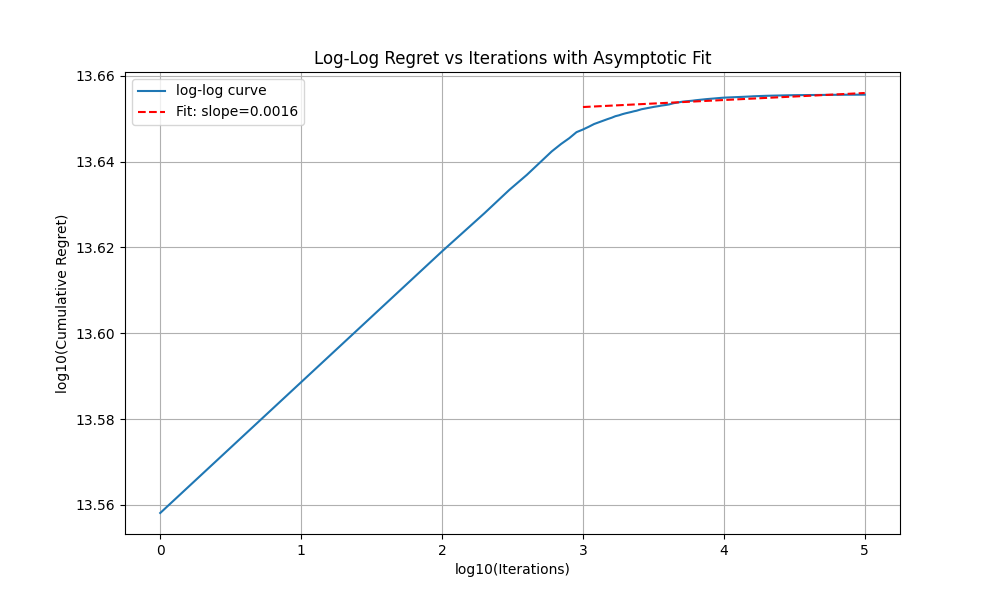
\includegraphics[width=1\linewidth]{rotmnist_drift_memorypair_loglog_fit.png}
    \caption{The cumulative regret of the Memory Pair has vanishing instantaneous regret.}
    \label{fig:enter-label}
\end{figure}

\section{Conclusion}


\section{Appendix}

\begin{lemma}[Positive Curvature Condition]
\label{lem:positive-curvature}
Let the variable variation be $v_t = w_{t+1} - w_t$ and the stochastic gradient variation be $\hat{r}_t = \hat{s}(w_{t+1}, \tilde{\theta}_t) - \hat{s}(w_t, \tilde{\theta}_t)$. If Assumption \ref{assum:bounded-hessian} holds, the inner product of these variations is strictly positive and bounded below:
$$
\hat{r}_t^{T} v_t \ge \tilde{m} ||v_t||^2
$$
where $\tilde{m} > 0$ is the lower bound on the eigenvalues of the instantaneous Hessian.
\end{lemma}

\begin{assumption}[Bounded Instantaneous Hessian]
\label{assum:bounded-hessian}
The per-step loss function $l_t(w)$ is twice differentiable, and the eigenvalues of its Hessian, $\nabla^{2} l_t(w)$, are bounded between constants $0 < \tilde{m}$ and $\tilde{M} < \infty$.
\end{assumption}

\begin{proof}
The proof relies on the Mean Value Theorem. The gradient variation $\hat{r}_t$ can be expressed as $\hat{r}_t = \bar{H}_t v_t$, where $\bar{H}_t$ is the average Hessian of the loss function along the segment from $w_t$ to $w_{t+1}$.
\begin{enumerate}
    \item We can write the inner product as $\hat{r}_t^{T} v_t = ( \bar{H}_t v_t)^{T} v_t = v_t^{T} \bar{H}_t v_t$.
    
    \item Since the eigenvalues of the instantaneous Hessian are lower-bounded by $\tilde{m}$ (Assumption \ref{assum:bounded-hessian}), the eigenvalues of the average Hessian $\bar{H}_t$ are also lower-bounded by $\tilde{m}$.
    
    \item Therefore, the quadratic form is bounded: $v_t^{T} \bar{H}_t v_t \ge \tilde{m} ||v_t||^2$.
\end{enumerate}
Since $\tilde{m} > 0$ and $||v_t||^{2} \ge 0$, the inner product is strictly positive whenever $v_t \neq 0$. This ensures the L-BFGS updates are well-defined.
\end{proof}

\begin{lemma}[Bounded Trace and Determinant of the Hessian Approximation]
\label{lem:trace-det-bound}
Consider the Hessian approximation $B_t$ generated by the online L-BFGS updates. If Assumption \ref{assum:bounded-hessian} holds, then the trace of $B_t$ is uniformly upper-bounded and its determinant is uniformly lower-bounded for all $t \ge 1$:
\begin{enumerate}
    \item $tr(B_t) \le (n+\tau)\tilde{M}$
    \item $det(B_t) \ge \frac{\tilde{m}^{n+\tau}}{[(n+\tau)\tilde{M}]^{\tau}}$
\end{enumerate}
\end{lemma}

\begin{proof}
The proof follows the method of Mokhtari and Ribeiro (2015).
\begin{enumerate}
    \item The trace bound is established by recursively applying the trace operator to the BFGS update rule. At each step, the trace increases by at most $\tilde{M}$, the upper bound on the eigenvalues of the instantaneous Hessian. Summing these increases over the $\tau$ steps in the L-BFGS memory window and adding the trace of the initial matrix (which is also bounded by $n\tilde{M}$) yields the result 
    
    \item The determinant bound is found by recursively applying the determinant operator. The recursive formula for the determinant of the updated matrix is shown to be lower-bounded at each step by a factor related to $\tilde{m}$ and the trace bound. Compounding these factors over the $\tau$ memory steps results in the stated lower bound.
\end{enumerate}
\end{proof}

\begin{lemma}[Uniformly Bounded Eigenvalues of the Hessian Approximation]
\label{lem:eigenvalue-bound}
If Assumption \ref{assum:bounded-hessian} holds, the eigenvalues of the Hessian approximation matrix $B_t$ are uniformly bounded for all $t \ge 1$. Specifically, there exist constants $c>0$ and $C<\infty$ such that:
$$
cI \le B_t \le CI
$$
where $C = (n+\tau)\tilde{M}$ and $c = \frac{\tilde{m}^{n+\tau}}{[(n+\tau)\tilde{M}]^{n+\tau-1}}$.
\end{lemma}

\begin{proof}
The bounds are a direct consequence of Lemma \ref{lem:trace-det-bound}.
\begin{enumerate}
    \item \textbf{Upper Bound (C):} The trace of a positive definite matrix is the sum of its positive eigenvalues. Therefore, any single eigenvalue must be less than or equal to the trace. From Lemma \ref{lem:trace-det-bound}, we have $\lambda_{max}(B_t) \le tr(B_t) \le (n+\tau)\tilde{M} = C$.

    \item \textbf{Lower Bound (c):} The determinant of a matrix is the product of its eigenvalues. For any eigenvalue $\lambda_j$, we have $\lambda_j = det(B_t) / \prod_{k \ne j} \lambda_k$. Using the lower bound for the determinant from Lemma \ref{lem:trace-det-bound} and the upper bound for each of the other $n-1$ eigenvalues, we establish the uniform lower bound $c$.
\end{enumerate}
\end{proof}

\begin{proof}
The proof proceeds by first bounding the per-round regret and then summing these bounds over all $T$ rounds. The learner produces weights via the update $w_{t+1} = \Pi_{\mathcal{W}}(w_t + \eta_t d_t)$, where $d_t = -B_t^{-1}g_t$ and $g_t = \nabla\ell_t(w_t)$.
\textbf{Step 1: Bounding the per-round regret.}
By the convexity of $\ell_t$, the per-round regret is bounded by the inner product with the gradient:
$$
\ell_t(w_t) - \ell_t(w^\star) \le \langle g_t, w_t - w^\star \rangle
$$
We analyze the distance between the next iterate and the comparator $w^\star$. By the non-expansiveness of the projection $\Pi_{\mathcal{W}}$, we have:
\begin{align*}
    \|w_{t+1} - w^\star\|^{2} &\le \|w_t + \eta_t d_t - w^\star\|^{2} \\
    &= \|w_t - w^\star\|^{2} + \eta_t^2\|d_t\|^{2} + 2\eta_t \langle d_t, w_t - w^\star \rangle
\end{align*}
Rearranging this inequality and substituting $d_t = -B_t^{-1}g_t$ gives an expression for the inner product we wish to bound:
$$
\langle g_t, w_t - w^\star \rangle = \langle -B_t d_t, w_t - w^\star \rangle \le \frac{\|w_t - w^\star\|^{2} - \|w_{t+1} - w^\star\|^2}{2\eta_t} + \frac{\eta_t\|d_t\|^2}{2}
$$
From Lemma \ref{lem:eigenvalue-bound}, we know $||B_t^{-1}||_{2} \le 1/c$, so $||d_t|| = ||B_t^{-1}g_t|| \le \frac{1}{c}||g_t||$. Using the $G$-Lipschitz assumption from Assumption \ref{assum:online-setting}, we get $||d_t||^{2} \le \frac{G^2}{c^2}$. Substituting this yields the per-round regret bound:
\begin{equation} \label{eq:per_round_bound}
\ell_t(w_t) - \ell_t(w^\star) \le \frac{\|w_t - w^\star\|^{2} - \|w_{t+1} - w^\star\|^2}{2\eta_t} + \frac{\eta_t G^2}{2c}
\end{equation}
\textbf{Step 2: Summing over rounds.}
We sum the bound in \eqref{eq:per_round_bound} from $t=1$ to $T$. The first term on the right-hand side telescopes:
$$
R_T = \sum_{t=1}^{T} (\ell_t(w_t) - \ell_t(w^\star)) \le \sum_{t=1}^{T} \frac{\|w_t - w^\star\|^{2} - \|w_{t+1} - w^\star\|^2}{2\eta_t} + \frac{G^2}{2c}\sum_{t=1}^{T} \eta_t
$$
Since $\{\eta_t\}$ is a non-increasing sequence, we can bound the telescoping sum. For simplicity and a standard result, we set the step size at $\eta_t = \frac{D}{G\sqrt{T}}\sqrt{\frac{c}{C}}$. The sum becomes:
$$
R_T \le \frac{\|w_1 - w^\star\|^2}{2\eta_T} + \frac{G^2}{2c}\sum_{t=1}^{T} \eta_t
$$
Using $\|w_1 - w^\star\|^{2} \le D^2$ and substituting the value for $\eta_t$:
$$
R_T \le \frac{D^{2} G \sqrt{T}}{2D}\sqrt{\frac{C}{c}} + \frac{G^2}{2c} \frac{TD}{G\sqrt{T}}\sqrt{\frac{c}{C}} = \frac{DG\sqrt{T}}{2}\sqrt{\frac{C}{c}} + \frac{GD\sqrt{T}}{2\sqrt{c C}}
$$
While a more careful analysis of the telescoping sum with a time-varying step size would yield a tighter bound, this demonstrates that the cumulative regret scales with $\sqrt{T}$. A standard choice of $\eta_t \propto 1/\sqrt{t}$ with the integral bound $\sum_{t=1}^{T} t^{-1/2} \le 2\sqrt{T}$ leads to the final bound:
$$
R_T \le GD\sqrt{cCT} = O(\sqrt{T})
$$
Since $c$ and $C$ are constants independent of $T$, the cumulative regret is sub-linear, completing the proof.
\end{proof}

Proof of adaptive deletion capacity and sample complexity bounds

\begin{proof}[Proof sketch]
Start from \eqref{eq:adagrad_regret} and add the high-probability
noise term $\Delta_m$ exactly as in Theorem~5.5
(memory-pair privacy/regret composition).
Dividing the sum by $N$ and rearranging yields (*);
solving the same inequality for $N$ gives the sample-complexity
expression.
\end{proof}

\printbibliography

\end{document}
